\documentclass[a4 paper]{article}
% Set target color model to RGB
\usepackage[inner=2.0cm,outer=2.0cm,top=2.5cm,bottom=2.5cm]{geometry}
\usepackage{setspace}
\usepackage[rgb]{xcolor}
\usepackage{verbatim}
\usepackage{subcaption}
\usepackage{amsgen,amsmath,amstext,amsbsy,amsopn,tikz,amssymb}
\usepackage{fancyhdr}
\usepackage[colorlinks=true, urlcolor=blue,  linkcolor=blue, citecolor=blue]{hyperref}
\usepackage[colorinlistoftodos]{todonotes}
\usepackage{rotating}
\usepackage{tikz}
\usetikzlibrary{decorations.pathreplacing} 
\usetikzlibrary{bayesnet} 

\usepackage{float}
\usepackage{minted}


%\usetikzlibrary{through,backgrounds}
\hypersetup{%
pdfauthor={Ashudeep Singh},%
pdftitle={Homework},%
pdfkeywords={Tikz,latex,bootstrap,uncertaintes},%
pdfcreator={PDFLaTeX},%
pdfproducer={PDFLaTeX},%
}
%\usetikzlibrary{shadows}
% \usepackage[francais]{babel}
\usepackage{booktabs}
\newcommand{\ra}[1]{\renewcommand{\arraystretch}{#1}}

\newtheorem{thm}{Theorem}[section]
\newtheorem{prop}[thm]{Proposition}
\newtheorem{lem}[thm]{Lemma}
\newtheorem{cor}[thm]{Corollary}
\newtheorem{defn}[thm]{Definition}
\newtheorem{rem}[thm]{Remark}
\numberwithin{equation}{section}

\newcommand{\homework}[7]{
   \pagestyle{myheadings}
   \thispagestyle{plain}
   \newpage
   \setcounter{page}{1}
   \noindent
   \begin{center}
   \framebox{
      \vbox{\vspace{2mm}
    \hbox to 6.28in { {\bf 67800 - Probabilistic Methods in Artificial Intelligence \hfill {\small (#2)}} }
       \vspace{6mm}
       \hbox to 6.28in { {\Large \hfill #1  \hfill} }
       \vspace{6mm}
       \hbox to 6.28in { {\it Instructor: {\rm #3} \hfill TA: {\rm #5} \hfill Name: {\rm #6} {\rm #7}} }
       %\hbox to 6.28in { {\it TA: #4  \hfill #6}}
      \vspace{2mm}}
   }
   \end{center}
   \markboth{#6 -- #1}{#6 -- #1}
   \vspace*{4mm}
}

\newcommand{\problempoints}[2]{~\\\fbox{\textbf{Problem #1}}\hfill (#2 points)\newline\newline}
\newcommand{\subproblem}[1]{~\newline\textbf{(#1)}}
\newcommand{\D}{\mathcal{D}}
\newcommand{\Hy}{\mathcal{H}}
\newcommand{\VS}{\textrm{VS}}
\newcommand{\solution}{~\newline\textbf{\textit{(Solution)}} }

\newcommand{\important}[1]{\textcolor{blue}{\textit{\textbf{#1}}}} 

\newcommand{\problem}[1]{~\\\fbox{\textbf{Problem #1}} \newline\newline}


\newcommand{\bbF}{\mathbb{F}}
\newcommand{\bbX}{\mathbb{X}}
\newcommand{\bI}{\mathbf{I}}
\newcommand{\bX}{\mathbf{X}}
\newcommand{\bY}{\mathbf{Y}}
\newcommand{\bepsilon}{\boldsymbol{\epsilon}}
\newcommand{\balpha}{\boldsymbol{\alpha}}
\newcommand{\bbeta}{\boldsymbol{\beta}}
\newcommand{\0}{\mathbf{0}}

\setlength{\parindent}{0pt}


\begin{document}
\homework{Project 2 - Inference}{Due: 27/06/24}{Prof. Gal Elidan}{}{Ela Fallik}{Hadar Tal}{}


\section*{Part I: Theoretical Questions}

\subsection*{1. Extreme Cases of the Mutilated Network}

\subsubsection*{\tblu{1.1 Assuming we see evidence \( e_r = \{M = m_0, F = f_1\} \)}}

\begin{enumerate}
    \item[(a)] \tblu{What is the graph of the mutilated network \( B_{e_r} \)? Which CPDs have changed?}
    
    \item[(b)] \tblu{Show that the proposal distribution is equal to the posterior \( p_B(X \mid e_r) \) in this case.}
    
    \item[(c)] \tblu{What are the IS weights?}
    
    \item[(d)] \tblu{Is \( q = p_{B_e} \) a good choice for the proposal distribution in this case?}
\end{enumerate}

\subsubsection*{\tblu{1.2 Assuming we see evidence \( e_l = \{n = n_1, L = l_1\} \)}}

\begin{enumerate}
    \item[(a)] \tblu{What is the graph of the mutilated network \( B_{e_l} \)? Which CPDs have changed?}
    
    \item[(b)] \tblu{Show that the proposal distribution is equal to the prior \( p_B(X) \) in this case.}
    
    \item[(c)] \tblu{What are the IS weights?}
    
    \item[(d)] \tblu{Is \( q = p_{B_e} \) a good choice for the proposal distribution in this case?}
\end{enumerate}

\subsubsection*{\tblu{1.3 Conclusion}}

\tblu{Use these two extreme cases to conclude, for a general BN, when \( q = p_{B_e} \) will be a good proposal distribution.}






\newpage
\subsection*{2. Data Association}

\begin{enumerate}
    \item \tblu{Compute the acceptance probability \( A(c, c') \) for each MH step.}
    
    The acceptance probability \( A(c, c') \) for transitioning from state \( c \) to \( c' \) is given by:
    \[
    A(c \to c') = \min \left( 1, \frac{\pi(c') T(c' \to c)}{\pi(c) T(c \to c')} \right)
    \]
    where:
    \begin{itemize}
        \item \( \pi(c) \) is the target distribution at state \( c \).
        \item \( T(c \to c') \) is the proposal distribution for moving from state \( c \) to state \( c' \).
    \end{itemize}

    In our case, the target distribution \( \pi(c) \) is the posterior \( p(c \mid v_1, \ldots, v_K) \), which can be expressed using Bayes' theorem as:
    \[
    p(c \mid v_1, \ldots, v_K) = \frac{p(v_1, \ldots, v_K \mid c) p(c)}{p(v_1, \ldots, v_K)}
    \]
    Since \( p(v_1, \ldots, v_K) \) is a normalizing constant and does not affect the ratio, it can be ignored for the acceptance probability calculation. Thus, we have:
    \[
    \frac{p(c' \mid v_1, \ldots, v_K)}{p(c \mid v_1, \ldots, v_K)} = \frac{p(v_1, \ldots, v_K \mid c') p(c')}{p(v_1, \ldots, v_K \mid c) p(c)}
    \]

    Assuming a uniform prior \( p(c) \) over all permutations:
    \[
    p(c) = p(c') \implies \frac{p(c')}{p(c)} = 1
    \]

    Therefore, the acceptance probability simplifies to:
    \[
    A(c \to c') = \min \left( 1, \frac{p(v_1, \ldots, v_K \mid c')}{p(v_1, \ldots, v_K \mid c)} \cdot \frac{T(c' \to c)}{T(c \to c')} \right)
     \stackrel{\text{uniform transition}}{=} \min \left( 1, \frac{p(v_1, \ldots, v_K \mid c')}{p(v_1, \ldots, v_K \mid c)} \right)
    \]

    Given the independence of observations given the correspondences:
    \[
    p(v_1, \ldots, v_K \mid c) = \prod_{i=1}^{K} p(V_i \mid C_i = c_i)
    \]

    Thus, the acceptance probability can be expressed as:
    \[
    A(c \to c') = \min \left( 1, \frac{\prod_{i=1}^{K} p(V_i \mid C_i = c'_i)}{\prod_{i=1}^{K} p(V_i \mid C_i = c_i)} \right)
    \]

    Since \( c \) and \( c' \) differ only by the swap of two correspondence variables \( C_i \) and \( C_j \), for most objects, 
    the terms in the numerator and denominator cancel out, except for \( V_i \) and \( V_j \). Therefore, the formula simplifies to:
    \[
    A(c \to c') = \min \left( 1, \frac{p(V_i \mid C_i = c'_i) \cdot p(V_j \mid C_j = c'_j)}{p(V_i \mid C_i = c_i) \cdot p(V_j \mid C_j = c_j)} \right)
    \]

    This simplification arises because \( c \) and \( c' \) differ only in the assignments of \( C_i \) and \( C_j \). The proposal distribution is symmetric, meaning \( T(c \to c') = T(c' \to c) \). Therefore, the acceptance probability further simplifies to:
    \[
    A(c \to c') = \min \left( 1, \frac{p(V_i \mid C_i = c'_i) \cdot p(V_j \mid C_j = c'_j)}{p(V_i \mid C_i = c_i) \cdot p(V_j \mid C_j = c_j)} \right)
    \]

    This formula gives us the acceptance probability for each MH step, ensuring the correctness and convergence of the algorithm.

    
    \newpage
    \item \tblu{Suppose we have run the MH sampler for a long time and collected \( M \) samples \( \{(C_1^{[m]}, \ldots, C_K^{[m]})\}_{m=T+1}^{T+M} \) 
    after the chain has mixed. Give an explicit expression for estimating the posterior \( p(C_i \mid v_1, \ldots, v_K) \).}
       
    The posterior probability \( p(C_i = k \mid v_1, \ldots, v_K) \) for a specific correspondence variable \( C_i \) taking the value \( k \) can be estimated as the fraction of samples where \( C_i = k \). Mathematically, this is given by:
    \[
    p(C_i = k \mid v_1, \ldots, v_K) \approx \frac{1}{M} \sum_{m=T+1}^{T+M} \delta(C_i^{[m]}, k)
    \]
    where \( \delta(C_i^{[m]}, k) \) is the Kronecker delta function, defined as:
    \[
    \delta(C_i^{[m]}, k) =
    \begin{cases}
    1 & \text{if } C_i^{[m]} = k \\
    0 & \text{if } C_i^{[m]} \neq k
    \end{cases}
    \]

    Thus, the posterior distribution \( p(C_i \mid v_1, \ldots, v_K) \) can be estimated as:
    \[
    p(C_i \mid v_1, \ldots, v_K) \approx \left\{ \frac{1}{M} \sum_{m=T+1}^{T+M} \delta(C_i^{[m]}, k) \right\}_{k=1}^{K}
    \]

    This expression gives an explicit method for estimating the posterior distribution of the correspondence variables after collecting \( M \) 
    samples from the MH sampler, leveraging the convergence property of MC (which converges to the true posterior as \( M \to \infty \)).


    \item \tblu{Your fellow student hears about your MH algorithm and suggests that you can also consider using Gibbs sampling to compute your marginals. Will this work? Explain.}
    
    consider \( K = 2 \).

    The possible states are:
    \[
    c_1 = (1, 2), \quad c_2 = (2, 1)
    \]
    
    In Gibbs sampling, each variable is updated in turn by sampling from its conditional distribution given the other variables. Suppose we start in state \( c_1 = (1, 2) \). When we update \( C_1 \), we sample from \( p(C_1 \mid C_2 = 2) \). Since \( C_2 = 2 \), \( C_1 \) must be 1, so no change occurs. Similarly, updating \( C_2 \) by sampling from \( p(C_2 \mid C_1 = 1) \) keeps \( C_2 \) at 2. Thus, the state remains \( c_1 = (1, 2) \).
    
    If we start in state \( c_2 = (2, 1) \), updating \( C_1 \) by sampling from \( p(C_1 \mid C_2 = 1) \) keeps \( C_1 \) at 2, and updating \( C_2 \) by sampling from \( p(C_2 \mid C_1 = 2) \) keeps \( C_2 \) at 1. Thus, the state remains \( c_2 = (2, 1) \).
    
    This shows that Gibbs sampling gets stuck in the initial state and cannot transition between \( (1, 2) \) and \( (2, 1) \). Therefore, the process is not irreducible.
    
    For larger \( K \), the situation remains similar. If \( K \) is even, Gibbs sampling can only reach even permutations (those that can be achieved by an even number of swaps), and if \( K \) is odd, it can only reach odd permutations. This restricts the state space significantly.
    
    In contrast, the Metropolis-Hastings algorithm with the swap proposal can move between any states, ensuring irreducibility and the ability to explore the entire state space.
    
    Thus, Gibbs sampling will not work for this data association problem, whereas the Metropolis-Hastings algorithm is appropriate.

\end{enumerate}






\newpage
\subsection*{3. Block Gibbs}


\begin{enumerate}
    \item \tblu{What will happen if we try to use Gibbs sampling on \( B \) to estimate \( p(x^1 \mid z^1) \)?}
    
    When using Gibbs sampling on the BN \( B \) to estimate \( p(x^1 \mid z^1) \), we update each variable in turn by sampling from its 
    conditional distribution given the current values of the other variables.

    The conditional distributions are as follows:
    \[
    \begin{aligned}
        p(X \mid Y, Z) &= 
        \begin{cases} 
        1 & \text{if } Z = X \oplus Y \\
        0 & \text{otherwise} 
        \end{cases} \\
        p(Y \mid X, Z) &= 
        \begin{cases} 
        1 & \text{if } Z = X \oplus Y \\
        0 & \text{otherwise} 
        \end{cases} \\
        p(Z \mid X, Y) &= 
        \begin{cases} 
        1 & \text{if } Z = X \oplus Y \\
        0 & \text{otherwise} 
        \end{cases}
    \end{aligned}
    \]

    Given \( Z = 1 \), we need to estimate \( p(X = 1 \mid Z = 1) \).

    1. \textbf{Initialization} : Assume we start with an initial state where \( (X, Y, Z) = (0, 1, 1) \).

    2. \textbf{Gibbs Sampling Iterations} : 
    \begin{itemize}
        \item Update \( X \) given \( Y \) and \( Z \):
            \[
            p(X = 1 \mid Y = 1, Z = 1) = 
            \begin{cases} 
            1 & \text{if } 1 = 1 \oplus 1 \\ 
            0 & \text{otherwise} 
            \end{cases} \Rightarrow X = 0
            \]
        \item Update \( Y \) given \( X \) and \( Z \):
            \[
            p(Y = 0 \mid X = 0, Z = 1) = 
            \begin{cases} 
            1 & \text{if } 1 = 0 \oplus 1 \\
            0 & \text{otherwise}
            \end{cases} \Rightarrow Y = 1
            \]

        \item Update \( Z \) given \( X \) and \( Y \):
            \[
            p(Z = 1 \mid X = 0, Y = 1) = 
            \begin{cases} 
            1 & \text{if } 1 = 0 \oplus 1 \\
            0 & \text{otherwise}
            \end{cases} \Rightarrow Z = 1
            \]
    \end{itemize}


    3. \textbf{Cycle Repetition} : The process will keep the variables in the same state: \( (X, Y, Z) = (0, 1, 1) \).

    This shows that Gibbs sampling gets stuck in a state where the variables do not change, because the deterministic nature of the XOR function does not allow for transitions between different states. Therefore, Gibbs sampling fails to explore the state space effectively in this scenario and cannot estimate \( p(x^1 \mid z^1) \) properly.

    \newpage
    \item \tblu{Now suppose we make \( Z \) a noisy XOR of its parents. Specifically,
    \[
    p(z_1 \mid X, Y) =
    \begin{cases}
    \epsilon & \text{if } x = 0, y = 0 \\
    1 - \epsilon & \text{if } x = 0, y = 1 \\
    1 - \epsilon & \text{if } x = 1, y = 0 \\
    \epsilon & \text{if } x = 1, y = 1
    \end{cases}
    \]
    What is the expected number of iterations until a state transition (i.e., from one state of the chain - some instantiation \( x, y, z \) - to a different state) 
    as a function of \( \epsilon \)? What can you conclude about problems that Gibbs sampling might encounter in this scenario?}
    

    To find the expected number of iterations until a state transition, we need to compute the transition probabilities and analyze the resulting Markov chain.

    \begin{enumerate}
        \item \textbf{Transition Probabilities:}
        \begin{itemize}
            \item If \( Z = X \oplus Y \):
            \[
            p(\text{transition}) = p(Z \ne X \oplus Y) 
            \]
            Given \( X \) and \( Y \) are uniformly distributed,
            \[
            p(Z \ne X \oplus Y) = \sum_{x,y} p(x, y) p(Z \ne X \oplus Y \mid x, y)
            \]
            \[
            = \frac{1}{4} \left( p(Z = 1 \mid (0, 0)) + p(Z = 0 \mid (0, 1)) + p(Z = 0 \mid (1, 0)) + p(Z = 1 \mid (1, 1)) \right) = \frac{1}{4} (4\epsilon) = \epsilon
            \]
    
            \item If \( Z \ne X \oplus Y \):
            \[
            p(\text{transition}) = p(Z = X \oplus Y) = 1 - \epsilon
            \]
        \end{itemize}
    
        \item \textbf{Markov Chain Analysis:}
        \begin{itemize}
            \item Define states \( A \) and \( B \):
            \[
            A: Z = X \oplus Y, \quad B: Z \ne X \oplus Y
            \]
            \[
            p(A \to B) = \epsilon, \quad p(B \to A) = 1 - \epsilon
            \]
    
            \item Stationary Distribution:
            \[
            \pi(A) + \pi(B) = 1
            \]
            Using the balance equations:
            \[
            \pi(A) = (1 - \epsilon) \pi(A) + \epsilon \pi(B)
            \]
            Since \(\pi(A) + \pi(B) = 1\):
            \[
            \pi(A) = (1 - \epsilon) \pi(A) + \epsilon (1 - \pi(A))
            \]
            \[
            \pi(A) = (1 - \epsilon) \pi(A) + \epsilon - \epsilon \pi(A)
            \]
            \[
            \pi(A) = \pi(A) (1 - \epsilon - \epsilon) + \epsilon
            \]
            \[
            \pi(A) (1 - \epsilon + \epsilon) = \epsilon
            \]
            \[
            \pi(A) = 1 - \epsilon
            \]
            Therefore:
            \[
            \pi(B) = \epsilon
            \]
    
            \item Expected Number of Iterations:
            The expected number of iterations \( \mathbb{E}(\text{iterations}) \) until a state transition can be computed using the law of total expectation. Let \( T \) be the random variable representing the number of iterations until a state transition.
            
            Using the stationary distribution, we can write:
            \[
            \mathbb{E}[T] = \pi(A) \cdot \mathbb{E}[T \mid S = A] + \pi(B) \cdot \mathbb{E}[T \mid S = B]
            \]
            
            Since the time to transition from state \( A \) to \( B \) is geometrically distributed with parameter \( \epsilon \), the expected number of steps is \( \frac{1}{\epsilon} \). Similarly, the time to transition from state \( B \) to \( A \) is geometrically distributed with parameter \( 1 - \epsilon \), so the expected number of steps is \( \frac{1}{1 - \epsilon} \):
            \[
            \mathbb{E}[T \mid S = A] = \frac{1}{\epsilon}, \quad \mathbb{E}[T \mid S = B] = \frac{1}{1 - \epsilon}
            \]
            
            Therefore:
            \[
            \mathbb{E}[T] = (1 - \epsilon) \cdot \frac{1}{\epsilon} + \epsilon \cdot \frac{1}{1 - \epsilon} = 
            \]
            \[
            = \frac{1 - \epsilon}{\epsilon} + \frac{\epsilon}{1 - \epsilon}
            \]
            \[
            = \frac{(1 - \epsilon)^2 + \epsilon^2}{\epsilon (1 - \epsilon)} = \frac{1 - 2\epsilon + \epsilon^2 + \epsilon^2}{\epsilon (1 - \epsilon)} = \frac{1 - 2\epsilon + 2\epsilon^2}{\epsilon - \epsilon^2}
            \]
        \end{itemize}

        \item \textbf{Conclusion:}
        Gibbs sampling might encounter issues if \( \epsilon \) is very small or very close to 1.
        In these cases, \( Z \) will rarely change its value, leading to very slow mixing of the Markov chain and making Gibbs sampling inefficient
        (the limit of the expected number of iterations as \( \epsilon \) approaches 0 or 1 is infinity).
        \begin{itemize}
            \item When \( \epsilon \) is close to 0.5, the chain will mix more rapidly.
            \item Therefore, the efficiency of Gibbs sampling in this scenario is highly dependent on the value of \( \epsilon \). For very small or very large \( \epsilon \), the chain will take a long time to transition between states, resulting in poor performance of Gibbs sampling.
        \end{itemize}

    \end{enumerate}
    


    \item \tblu{Alternatively, we can think of a variant of Gibbs sampling where larger steps are taken. 
    Specifically, larger sets of variables are sampled simultaneously while the rest are fixed. 
    Show that sampling two variables given the third overcomes the problem of Gibbs sampling in the deterministic XOR network.}
    
    \begin{itemize}
        \item Instead of sampling one variable at a time, we sample two variables simultaneously given the value of the third variable. This breaks the deterministic dependency and allows transitions between states that would otherwise be impossible.

        \item \textbf{Steps:}
        \begin{enumerate}
            \item Fix the value of \( Z \).
            \item Sample \( (X, Y) \) given \( Z \).
        \end{enumerate}

        \item \textbf{Transition Probabilities:}
        \begin{itemize}
            \item Given \( Z \), the possible values of \( (X, Y) \) are:
            \[
            \begin{aligned}
                &\text{If } Z = 0: \quad (X, Y) = (0, 0) \text{ or } (1, 1) \text{ with equal probability} \\
                &\text{If } Z = 1: \quad (X, Y) = (0, 1) \text{ or } (1, 0) \text{ with equal probability}
            \end{aligned}
            \]

            \item By sampling \( (X, Y) \) given \( Z \), we can transition between the states efficiently. The deterministic dependency of \( Z \) on \( X \) and \( Y \) is no longer a hindrance because we are not attempting to change one variable while holding the other constant.
        \end{itemize}

        \item \textbf{Justification:}
        \begin{itemize}
            \item The main issue with standard Gibbs sampling is that it gets stuck in configurations where a single-variable update cannot change the state due to the XOR constraint. By sampling pairs of variables, we allow transitions that respect the XOR constraint directly.
            \item This method ensures that the Markov chain can explore the entire state space because any valid combination of \( (X, Y, Z) \) can be reached by fixing \( Z \) and sampling \( (X, Y) \).
            \item The resulting Markov chain is irreducible and aperiodic, ensuring convergence to the correct stationary distribution.
        \end{itemize}
    \end{itemize}





    \newpage
    \item \tblu{To use this last sampler, we need to calculate the probability of a pair of variables given the rest. 
    Write down a (simplified as possible) formula for \( p_{\Phi}(X_i, X_j \mid X \setminus \{X_i, X_j\}) \) for a general Gibbs distribution \( p_{\Phi} \).}


 
\textbf{Derivation:}
Consider a general Gibbs distribution \( p_\Phi \) defined over a set of random variables \( \mathcal{X} = \{X_1, X_2, \ldots, X_n\} \). The Gibbs distribution is given by:
\[
P_\mathcal{X}(x_1, x_2, \ldots, x_n) = \frac{1}{Z} \prod_{j} \phi_j(X_{c_j})
\]
where:
\begin{itemize}
    \item \( \mathcal{C} = \{c_1, c_2, \ldots, c_m\} \) is a set of cliques in the graph.
    \item \( X_{c_j} \) is the set of random variables in clique \( c_j \).
    \item \( \phi_j : \text{Val}(X_{c_j}) \to \mathbb{R}^+ \) is a potential function / factor over the clique \( c_j \).
    \item \( Z \) is the normalization constant (partition function).
\end{itemize}

\begin{enumerate}
    \item \textbf{Joint Distribution:}
    The joint distribution \( P_\mathcal{X}(X_1, X_2, \ldots, X_n) \) can be written as:
    \[
    P_\mathcal{X}(X_1, X_2, \ldots, X_n) = \frac{1}{Z} \prod_{j} \phi_j(X_{c_j})
    \]

    \item \textbf{Conditional Distribution:}
    The conditional distribution \( p_\Phi(X_i, X_j \mid \mathcal{X} \setminus \{X_i, X_j\}) \) is given by:
    \[
    p_\Phi(X_i, X_j \mid \mathcal{X} \setminus \{X_i, X_j\}) = \frac{P_\mathcal{X}(X_i, X_j, \mathcal{X} \setminus \{X_i, X_j\})}{P_\mathcal{X}(\mathcal{X} \setminus \{X_i, X_j\})}
    \]
    
    \item \textbf{Simplification:}
    Using the definition of the Gibbs distribution, we can write:
    \begin{align*}
        p_\Phi(X_i, X_j \mid \mathcal{X} \setminus \{X_i, X_j\}) &= \frac{\frac{1}{Z} \prod_{j} \phi_j(X_{c_j})}{\sum_{X_i, X_j} \frac{1}{Z} \prod_{j} \phi_j(X_{c_j})} \\
        &= \frac{\prod_{j} \phi_j(X_{c_j})}{\sum_{X_i, X_j} \prod_{j} \phi_j(X_{c_j})} \\
        &= \frac{\prod_{j: X_{c_j} \cap \{X_i, X_j\} \ne \emptyset} \phi_j(X_{c_j}) \prod_{k: X_{c_k} \cap \{X_i, X_j\} = \emptyset} \phi_k(X_{c_k})}{\sum_{X_i, X_j} \prod_{j: X_{c_j} \cap \{X_i, X_j\} \ne \emptyset} \phi_j(X_{c_j}) \prod_{k: X_{c_k} \cap \{X_i, X_j\} = \emptyset} \phi_k(X_{c_k})} \\
        &= \frac{\prod_{j: X_{c_j} \cap \{X_i, X_j\} \ne \emptyset} \phi_j(X_{c_j})}{\sum_{X_i, X_j} \prod_{j: X_{c_j} \cap \{X_i, X_j\} \ne \emptyset} \phi_j(X_{c_j})}
    \end{align*}

\end{enumerate}

\textbf{Conclusion:}
The simplified formula for the conditional distribution of a pair of variables given the rest in a general Gibbs distribution \( p_\Phi \) is:
\[
p_\Phi(X_i, X_j \mid \mathcal{X} \setminus \{X_i, X_j\}) = \frac{\prod_{j: X_{c_j} \cap \{X_i, X_j\} \ne \emptyset} \phi_j(X_{c_j})}{\sum_{X_i, X_j} \prod_{j: X_{c_j} \cap \{X_i, X_j\} \ne \emptyset} \phi_j(X_{c_j})}
\]

\end{enumerate}



\newpage
\subsection*{4. Collapsed Particles}


\begin{enumerate}
    \item \tblu{Show that
    \[
    E_{p(X \mid e)}[f(X)] = \sum_{x_p} p(x_p \mid e) E_{p(X_d \mid x_p, e)}[f(x_p, X_d, e)]
    \]
    Use this to explain how to estimate \( E_{p(X \mid e)}[f(X)] \) using the collapsed particles.}


    \textbf{Derivation:}
    \begin{align*}
    \mathbb{E}_{p(\mathcal{X} \mid e)} [f(\mathcal{X})] &= \sum_{\mathcal{X}} f(\mathcal{X}) p(\mathcal{X} \mid e) \\
    &\stackrel{\mathcal{X} = \mathcal{X}_d \sqcup \mathcal{X}_p }{=} \sum_{x_p \in \mathcal{X}_p} \sum_{x_d \in \mathcal{X}_d} f(x_p, x_d) p(x_p, x_d \mid e) \\
    &= \sum_{x_p \in \mathcal{X}_p} \left( \sum_{x_d \in \mathcal{X}_d} f(x_p, x_d) p(x_d \mid x_p, e) \right) p(x_p \mid e) \\
    &= \sum_{x_p \in \mathcal{X}_p} \mathbb{E}_{p(\mathcal{X}_d \mid x_p, e)} [f(x_p, \mathcal{X}_d)] p(x_p \mid e) \\
    &= \sum_{x_p \in \mathcal{X}_p} p(x_p \mid e) \mathbb{E}_{p(\mathcal{X}_d \mid x_p, e)} [f(x_p, \mathcal{X}_d)]
    \end{align*}

    
    \textbf{How to estimate \( \mathbb{E}_{p(\mathcal{X} \mid e)} [f(\mathcal{X})] \) using the collapsed particles:}
    \begin{itemize}
        \item Sample \( x_p \) from \( p(\mathcal{X}_p \mid e) \).
        \item For each sampled \( x_p \), compute the conditional expectation \( \mathbb{E}_{p(\mathcal{X}_d \mid x_p, e)} [f(x_p, \mathcal{X}_d)] \) (by IS).
        \item Average these conditional expectations weighted by \( p(x_p \mid e) \) (IS).
    \end{itemize}
    
    By using the collapsed particles, we effectively reduce the dimensionality of the problem, making the estimation more efficient while leveraging the known structure of the distribution \( p(\mathcal{X}_d \mid x_p, e) \).

    


    
    \item \tblu{Describe what this approach is equivalent to in the two extreme cases: When \( X_p = \emptyset \) and when \( X_p = X \).}
    
    \begin{itemize}
        \item \textbf{When \( \mathcal{X}_p = \emptyset \):}
        In this extreme case, there are no variables in the set \( \mathcal{X}_p \), which means we are not collapsing any variables. Consequently, all variables are in the set \( \mathcal{X}_d \). Therefore, the approach simplifies to directly estimating the expectation using importance sampling over the entire state space \( \mathcal{X} \):
    
        \begin{align*}
        \mathbb{E}_{p(\mathcal{X} \mid e)} [f(\mathcal{X})] &= \sum_{x_p \in \emptyset} p(x_p \mid e) \mathbb{E}_{p(\mathcal{X}_d \mid x_p, e)} [f(x_p, \mathcal{X}_d)] \\
        &= \mathbb{E}_{p(\mathcal{X}_d \mid e)} [f(\mathcal{X}_d)]
        \end{align*}
    
        In this scenario, we are simply performing standard importance sampling over the full state space \( \mathcal{X} \).
    
        \item \textbf{When \( \mathcal{X}_p = \mathcal{X} \):}
        In this extreme case, all variables are in the set \( \mathcal{X}_p \), which means \( \mathcal{X}_d = \emptyset \). Consequently, there are no variables left to be integrated out conditionally. The approach simplifies to:
    
        \begin{align*}
        \mathbb{E}_{p(\mathcal{X} \mid e)} [f(\mathcal{X})] &= \sum_{x_p \in \mathcal{X}} p(x_p \mid e) \mathbb{E}_{p(\emptyset \mid x_p, e)} [f(x_p, \emptyset)] \\
        &= \sum_{x_p \in \mathcal{X}} f(x_p) p(x_p \mid e) \\
        &= \mathbb{E}_{p(\mathcal{X} \mid e)} [f(\mathcal{X})]
        \end{align*}
    
        In this case, we are directly sampling from the full joint distribution without collapsing any variables, which is equivalent to direct sampling from \( p(\mathcal{X} \mid e) \).
    \end{itemize}
    
    In summary When \( \mathcal{X}_p \in \{\emptyset, \mathcal{X} \} \), the approach reduces to standard importance sampling over the entire state space \( \mathcal{X} \).

    


    \item \tblu{Describe what will be a good "rule-of-thumb" in choosing \( X_p \) and \( X_d \) for this method.}
    
    When choosing the sets \( \mathcal{X}_p \) and \( \mathcal{X}_d \) for collapsed particle sampling, it is essential to strike a balance that maximizes computational efficiency and sampling accuracy. Here are some rules of thumb:

    \begin{itemize}

        \item \textbf{Dependency Structure:} 
        If variables in \( \mathcal{X}_p \) are highly dependent on each other, sampling them together can reduce the variance of the estimator.
        Conversely, if variables in \( \mathcal{X}_d \) are conditionally independent given \( \mathcal{X}_p \), this simplifies the computation of \( \mathbb{E}_{p(\mathcal{X}_d \mid x_p, e)} [f(x_p, \mathcal{X}_d)] \).
    
        \item \textbf{Computational Efficiency:}
        Ensure that the sets \( \mathcal{X}_p \) and \( \mathcal{X}_d \) are of manageable size, as sampling and computing conditional expectations can be computationally expensive for large sets.
    
        \item \textbf{Practical Considerations:}
        - Choose \( \mathcal{X}_p \) such that the marginal distribution \( p(\mathcal{X}_p \mid e) \) is easy to estimate or sample from.
        - Choose \( \mathcal{X}_d \) so that efficient algorithms or approximations are available for computing \( \mathbb{E}_{p(\mathcal{X}_d \mid x_p, e)} [f(x_p, \mathcal{X}_d)] \).
    
    \end{itemize}



    \item \tblu{Give an example of a Bayesian Network over \( X \), a set of observed variables \( E \) and a query \( p(X \mid e) \) 
    that is hard to calculate directly, but can be estimated using the described method of collapsed particles using 
    efficient calculations only. \( X_d \) and \( X_p \) should be \( \neq \emptyset \) in your example.}
    



Consider a Bayesian Network with the following structure:

\begin{center}
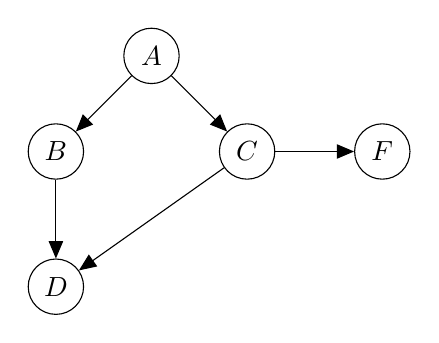
\begin{tikzpicture}
    % Nodes
    \node[latent] (A) {$A$};
    \node[latent, below left=of A] (B) {$B$};
    \node[latent, below right=of A] (C) {$C$};
    \node[latent, below=of B] (D) {$D$};
    \node[latent, right=of C] (F) {$F$};

    % Edges
    \edge {A} {B, C};
    \edge {B, C} {D};
    \edge {C} {F};
\end{tikzpicture}
\end{center}

Here:
\begin{itemize}
    \item \( A \) is the parent of \( B \) and \( C \).
    \item \( B \) and \( C \) are the parents of \( D \).
    \item \( C \) is the parent of \( F \).
\end{itemize}

Let the set of observed variables be \( E = \{D\} \), and the query is \( p(A, B, C, F \mid D) \).

Calculating \( p(A, B, C, F \mid D) \) directly is difficult due to the dependencies among the variables. However, we can use the collapsed particle method to make the computation more efficient.

\textbf{Choosing \( \mathcal{X}_p \) and \( \mathcal{X}_d \):} \\
- Let \( \mathcal{X}_p = \{A, C\} \) \\ 
- Let \( \mathcal{X}_d = \{B, F\} \) \\


\textbf{Calculation:} \\
    Sample \( (A, C) \) from the joint distribution \( p(A, C \mid D) \). This can be done by factorizing the joint distribution:
    \[
    p(A, C \mid D) = \frac{p(D \mid A, C) p(A) p(C \mid A)}{p(D)}
    \]
    where
    \[
    p(D) = \sum_{A, C} p(D \mid A, C) p(A) p(C)
    \]

    Given the structure of the network, \( D \) depends on \( B \) and \( C \), and \( B \) depends on \( A \). Thus, the conditional distribution \( p(D \mid A, C) \) can be computed using:
    \[
    p(D \mid A, C) = \sum_{B} p(D \mid B, C) p(B \mid A)
    \]

    Assuming we have observed \( D = d \), we can simplify the sampling from \( p(A, C \mid D) \) using the above factorization.

    Given the sampled values \( (A, C) \), we compute the conditional distribution \( p(B, F \mid A, C, D) \):
    \[
    p(B, F \mid A, C, D) = p(B \mid A) p(F \mid C)
    \]
    This simplifies the computation because \( B \) depends only on \( A \), and \( F \) depends only on \( C \) (given the observations there are no active trails between \( B \) and \( F \)).

\textbf{Efficient Calculation:}
By collapsing the variables \( A \) and \( C \) (sampling them directly), we reduce the complexity of the problem. This allows us to handle the dependencies more efficiently and compute the conditional expectations using the simpler structure of the network.

  




    \item \tblu{In many cases, sampling from \( p(X_p \mid e) \) is still hard. 
    We therefore want to build a (Normalized) Importance Sampling version of this method. 
    We do this by sampling \( x_p \) from a proposal distribution \( q(X_p) \) and using the weights
    \[
    w(x_p) = \frac{p(x_p, e)}{q(x_p)} = \frac{p(x_p, e_p) \cdot p(x_d \mid x_p, e_p)}{q(x_p)}
    \]
    where \( E_p = E \cap X_p \) and \( E_d = E \cap X_d \). Prove the correctness of this method. Specifically, show that \( E_q[w(x_p)] = p(e) \), 
    and conclude that this procedure gives an estimation of \( E_{p(X \mid e)}[f(X)] \).}
\end{enumerate}



















\newpage
\section*{Part II}
\textbf{Programming Assignment - Inference in HMM}


\subsection*{1. Exact inference using dynamic-programming (DP)}

\begin{enumerate}
    \item \tblu{You are supplied with code for the forward and backward algorithms. Use them to implement the \texttt{log\_posterior\_Xt} method in the HMM class.}
    
    \begin{align*}
        P(X_t = k \mid O_{1:t}) &= \frac{P(X_t = k, O_{1:t})}{P(O_{1:t})} = \frac{P(X_t = k, O_{1:t}) \cdot P(O_{t+1:T} \mid X_t = k)}{P(O_{1:T})} \\
        \log P(X_t = k \mid O_{1:t}) &= \log \left( \frac{P(X_t = k, O_{1:t}) \cdot P(O_{t+1:T} \mid X_t = k)}{P(O_{1:T})} \right) \\
        &= \log P(X_t = k, O_{1:t}) + \log P(O_{t+1:T} \mid X_t = k) - \log P(O_{1:T}) \\
        &= \mathcal{F}[t, k] + \mathcal{B}[t, k] - \text{log\_likelihood}(O_{1:T})
    \end{align*}

    Implemented the \texttt{log\_posterior\_Xt} method in the HMM class to calculate the log posterior $P(X_t = k \mid O_{1:t})$ for each $t$ and $k$.


    
    \item \tblu{Exact posteriors:
    We load the observations from \texttt{obs\_data.csv}, calculate the marginal posteriors for the 
    $N = 20$ observations in the dataset $p(X_t = 1 | o_{1:T}[i])$, and plot the prior distributions $p(X_t = 1)$ versus the 
    mean marginal posteriors $\mu_t = \frac{1}{N} \sum_{i=1}^{N} p(X_t = 1 | o_{1:T}[i])$ for each $t$. \\
    What are the differences and why do they exist? What does it suggest about the distribution from which the observations were sampled?}

    \begin{figure}[H]
        \centering
        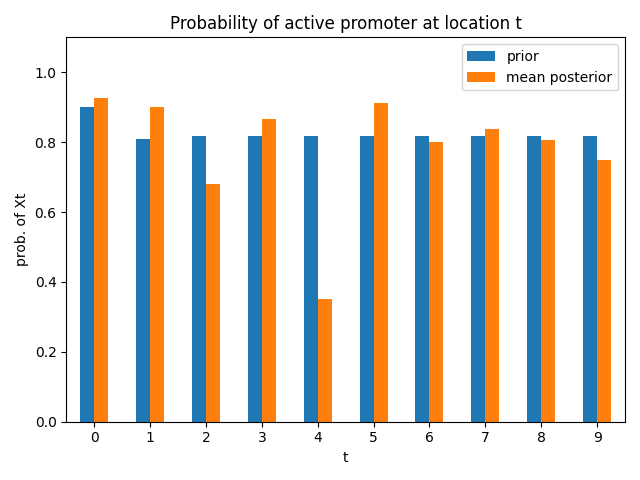
\includegraphics[width=0.4\textwidth]{../plots/q1_prior_vs_mean_posterior.png}
        \caption{Prior distributions $p(X_t = 1)$ versus the mean marginal posteriors $\mu_t = \frac{1}{N} \sum_{i=1}^{N} p(X_t = 1 | o_{1:T}[i])$ for each $t$.}
    \end{figure}

    
    The plot shows the prior distributions $p(X_t = 1)$ (blue bars) versus the mean marginal posteriors $\mu_t$ 
    (orange bars) for each time step $t$. The differences between the prior and the mean marginal posteriors suggest
     that the observations have a significant impact on the estimated probabilities of active promoters. 
     Specifically, the mean marginal posteriors differ from the prior distributions due to the evidence provided 
     by the observations. This indicates that the dataset likely contains informative observations that influence the 
     posterior estimates. \\
     The deviations from the prior suggest that the distribution from which the observations were sampled has regions with
      varying levels of promoter activity, as captured by the posterior probabilities.
    

    \item \tblu{We want to use the marginal posteriors $p(X_t | o_{1:T}[i])$ to assign each location $t$ its status and predict areas of active promoter:
    \[
    \hat{X}_t[i] = \arg\max_x p(X_t = x | o_{1:T}[i])
    \]
    Implement a \texttt{naive\_predict\_by\_posterior} method in the HMM class.}

    Implemented the \texttt{naive\_predict\_by\_posterior} method in the HMM class.
    

    \item \tblu{Prediction:
    We use this method to predict hidden sequences for the given observations. We compare them to the ground-truth sequences from \texttt{hidden\_data.csv}.
     What is the accuracy of these predictions (use the same definition as Project 1)? What is the difference compared to the prediction we used in Project 1?
      Is the rule in Eq.4 a good prediction rule?}

    \textbf{Results:}
    \begin{itemize}
        \item Exact Posterior Prediction Accuracy: 0.900
        \item Naive Prediction Accuracy: 0.895
    \end{itemize}
    
    \textbf{Analysis:}
    \begin{itemize}
        \item The exact posterior method is slightly more accurate than the naive method.
        \item The exact method uses the forward-backward algorithm, considering the entire observation sequence, 
            while the naive method likely uses a simpler, less contextual approach.
        \item This accuracy difference shows the exact posterior is better at capturing dependencies in the data.
        \item Eq. 4's rule is a good prediction method, leveraging the full observation sequence for more informed predictions.
    \end{itemize}

\end{enumerate}

\subsection*{2. Sampling-based inference}


\begin{enumerate}
    \item \tblu{Gibbs sampling: In this algorithm, we’ll start with a starting point $X_{1:T}$ sampled from the prior $p(X_{1:T})$, 
    and sample $M$ sequences of hidden states sequentially:
    \[
    X_t^{(m)} \sim p(X_t | X_{-t}^{(m-1)}, o_{1:T}[i]), \quad t = 1, \ldots, T
    \]
    We then use the samples to estimate the posterior $p(X_t = x | o_{1:T}[i])$ for each $t$.}
    
    \begin{enumerate}
        \item \tblu{For observations $o_{1:T}[i]$, at iteration $m$, we want to use the samples from the previous iteration 
        $\{X_t^{(m-1)}\}_{t=1}^{T}$ to sample $X_t^{(m)}$ from the distribution $p(X_t | X_{-t}^{(m-1)}, o_{1:T}[i])$. 
        How can we sample from this distribution using the CPDs of the network?} \\

        In a Hidden Markov Model (HMM), the Markov blanket of a hidden state $X_t$ includes its immediate neighbors and the observation at time $t$. Specifically, the Markov blanket of $X_t$ consists of $X_{t-1}$, $O_t$, and $X_{t+1}$ (if they exist). This is because in an HMM, $X_t$ is conditionally independent of all other variables given these three variables. 

        Given this, we can write the conditional distribution for sampling $X_t$ as follows:

        \begin{align*}
            &P(X_t = k \mid X_{-t}^{(m-1)}, O_{1:T}[i]) \\
            &= P(X_t = k \mid X_{t-1}^{(m-1)}, O_t[i], X_{t+1}^{(m-1)}) \\
            &= \frac{P_\phi(X_t = k, X_{t-1}^{(m-1)}, O_t[i], X_{t+1}^{(m-1)})}{\sum_{x_t \in \text{Val}(X_t)} P_\phi(X_t = x_t, X_{t-1}^{(m-1)}, O_t[i], X_{t+1}^{(m-1)})} \\
            &= \frac{P_\phi(X_{t-1}^{(m-1)}) \cdot P(X_t = k \mid X_{t-1}^{(m-1)}) \cdot P(O_t[i] \mid X_t = k) \cdot P(X_{t+1}^{(m-1)} \mid X_t = k)}{\sum_{x_t \in \text{Val}(X_t)} P_\phi(X_{t-1}^{(m-1)}) \cdot P(X_t = x_t \mid X_{t-1}^{(m-1)}) \cdot P(O_t[i] \mid X_t = x_t) \cdot P(X_{t+1}^{(m-1)} \mid X_t = x_t)} \\
            &= \frac{P(X_t = k \mid X_{t-1}^{(m-1)}) \cdot P(O_t[i] \mid X_t = k) \cdot P(X_{t+1}^{(m-1)} \mid X_t = k)}{\sum_{x_t \in \text{Val}(X_t)} P(X_t = x_t \mid X_{t-1}^{(m-1)}) \cdot P(O_t[i] \mid X_t = x_t) \cdot P(X_{t+1}^{(m-1)} \mid X_t = x_t)}
        \end{align*}

        
        \item \tblu{Given $M$ samples $\{X_t^{(m)}\}_{m=1}^{M}$ from the process described above, 
        how can we calculate the posterior $p(X_t = x | o_{1:T}[i])$, while discarding the first $M_{\text{start}}$ samples to allow for a “burn-in” period?}

        To calculate the posterior $p(X_t = x | o_{1:T}[i])$ for each $t$, we can use the samples $\{X_t^{(m)}\}_{m=M_{\text{start}}}^{M}$
        obtained from the Gibbs sampling process. 
        We can estimate the posterior by counting the number of times $X_t = x$ occurs in the samples and normalizing by the total number of samples. 
        The posterior can be calculated as follows:

        \[
        p(X_t = x | o_{1:T}[i]) = \frac{1}{M - M_{\text{start}}} \sum_{m=M_{\text{start}}}^{M} \mathbb{I}(X_t^{(m)} = x)
        \]

        where $\mathbb{I}(\cdot)$ is the indicator function that returns 1 if the condition is true and 0 otherwise.
        
        \item \tblu{Implement a method \texttt{gibbs\_sampling\_posterior} in the HMM class to calculate the posterior 
        $p(X_t = x | o_{1:T}[i])$ for each $t$ with $M - M_{\text{start}}$ samples.}
        

        Implemented the \texttt{gibbs\_sampling\_posterior} method in the HMM class.


        \item \tblu{We run the Gibbs algorithm with $M \in [10, 50, 70, 100, 200, 300, 500]$ samples to calculate the marginal 
        posteriors of each observation in the dataset. We run the algorithm 5 times for each value of $M$. 
        We plot the posterior of $X_5$ for the first 10 observations $p(X_5 | o_{1:T}[1 : 10])$ versus $M$ with confidence 
        intervals ($\mu \pm \sigma$), and add to the plot the exact posterior calculated using DP.
        Does the Gibbs estimation converge? Does it converge to the correct posterior? Explain your results. 
        What can you say about the convergence of this algorithm?}

        \begin{figure}[H]
            \centering
            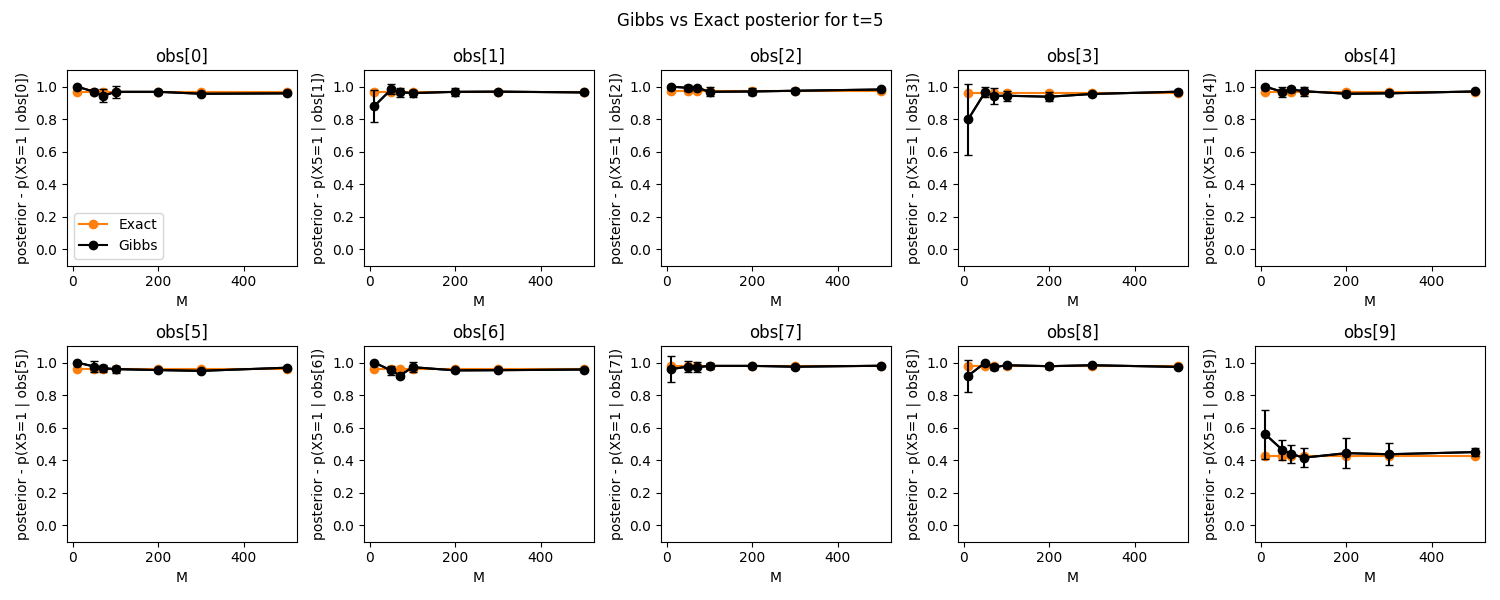
\includegraphics[width=0.9\textwidth]{../plots/Gibbs_est_vs_exact_posterior.png}
            \caption{Posterior of $X_5$ for the first 10 observations $p(X_5 | o_{1:T}[1 : 10])$ versus $M$ with confidence intervals ($\mu \pm \sigma$).}
        \end{figure}

        The plot shows the comparison between the Gibbs sampling estimation and the exact posterior calculated 
        using dynamic programming (DP) for $X_5$ across the first 10 observations. 

        \textbf{Analysis:}
        \begin{itemize}
            \item \textbf{Convergence:} The Gibbs estimation converges fairly fast as $M$ increases. Even with a relatively small number of samples (e.g., $M = 50$), the estimates are quite stable and close to the exact posterior.
            \item \textbf{Correctness:} The Gibbs estimates converge to values close to the exact posterior calculated using DP, indicating that the Gibbs sampling method is correctly estimating the posterior distributions.
            \item \textbf{Results:} The convergence of the Gibbs sampling algorithm demonstrates its effectiveness in approximating the true posterior distribution, especially with a higher number of samples $M$. The confidence intervals also decrease with increasing $M$, showing more precise estimates.
            \item \textbf{Implications:} The fast convergence of the Gibbs sampling method makes it a practical and efficient approach for posterior estimation in HMMs, providing reliable results with relatively few samples.
        \end{itemize}
        
    \end{enumerate}
    
    \item \tblu{We use the estimated posteriors of each algorithm and the \texttt{naive\_predict\_by\_posterior} method to assign 
    each location its status (same as for the exact posterior). We plot the accuracy of the algorithms as a function of $M$, 
    and plot on the same graph the accuracy of the exact posterior (as a constant function of $M$). What is the trend?}


    \begin{figure}[H]
        \centering
        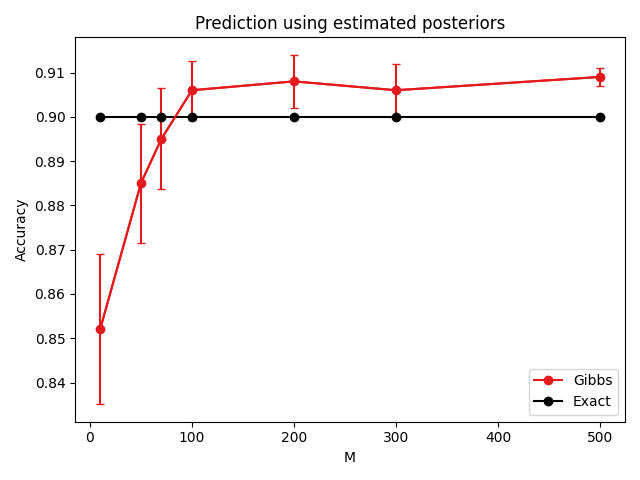
\includegraphics[width=0.6\textwidth]{../plots/est_vs_exact_accuracy.png}
        \caption{Accuracy of the algorithms as a function of $M$, with the accuracy of the exact posterior as a constant function of $M$.}
    \end{figure}

    The plot shows the accuracy of the Gibbs sampling algorithm compared to the exact posterior as a function of the number of samples $M$.

    \textbf{Analysis:}
    \begin{itemize}
        \item \textbf{Trend:} The accuracy of the Gibbs sampling algorithm increases rapidly with the number of samples $M$ and stabilizes around $M = 100$. The exact posterior accuracy remains constant.
        \item \textbf{Comparison:} The Gibbs sampling method eventually reaches and slightly surpasses the accuracy of the exact posterior, indicating that it is an effective method for estimating the posterior, especially with a larger number of samples.
        \item \textbf{Implications:} The Gibbs sampling method can achieve high accuracy with sufficient samples, making it a reliable alternative to exact inference methods. The slight fluctuation in accuracy with smaller $M$ values suggests that more samples are needed for stabilization.
    \end{itemize}

\end{enumerate}

\end{document}




